% !TeX program = xelatex
\documentclass[UTF8,a4paper,zihao=-4]{ctexart}

% =========================
% 基本宏包
% =========================
\usepackage[a4paper,left=2.7cm,right=2.7cm,top=2.6cm,bottom=2.6cm]{geometry}
\usepackage{amsmath,amssymb,bm}
\usepackage{booktabs}
\usepackage{array}
\usepackage{multirow}
\usepackage{longtable}
\usepackage{graphicx}
\graphicspath{{./}{doc/大作业/}}
\usepackage{xcolor}
\usepackage{float}
\usepackage{caption}
\usepackage{subcaption}
\usepackage{enumitem}
\usepackage{listings}
\usepackage{hyperref}
\usepackage{siunitx}
\usepackage{titlesec}
\usepackage{fancyhdr}
\usepackage{lastpage}

% =========================
% GB/T 3102.11-1993 数学排版约定
% 变量、变动附标和函数用斜体；
% 已定义算子、常数用正体。
% LaTeX 数学模式默认单字母变量为斜体；
% 本报告对算子使用 \mathrm 或 \operatorname。
% =========================
\newcommand{\dd}{\mathrm{d}}
\newcommand{\ee}{\mathrm{e}}
\newcommand{\T}{\mathrm{T}}
\newcommand{\diag}{\operatorname{diag}}
\newcommand{\tr}{\operatorname{tr}}
\newcommand{\rank}{\operatorname{rank}}
\newcommand{\Dmat}{\bm{D}}
\newcommand{\Bmat}{\bm{B}}
\newcommand{\Kmat}{\bm{K}}
\newcommand{\kmat}{\bm{k}}
\newcommand{\Tmat}{\bm{T}}
\newcommand{\Fvec}{\bm{F}}
\newcommand{\Uvec}{\bm{u}}
\newcommand{\epsvec}{\bm{\varepsilon}}
\newcommand{\sigvec}{\bm{\sigma}}

% =========================
% 颜色与超链接
% =========================
\definecolor{stapblue}{RGB}{34,78,140}
\definecolor{stapgray}{RGB}{245,246,248}
\definecolor{codegreen}{RGB}{0,110,60}
\definecolor{codepurple}{RGB}{120,40,120}

\hypersetup{
    colorlinks=true,
    linkcolor=stapblue,
    citecolor=stapblue,
    urlcolor=stapblue,
    pdftitle={STAP++程序研发报告},
    pdfauthor={请填写姓名}
}

% =========================
% 页眉页脚
% =========================
\pagestyle{fancy}
\fancyhf{}
\setlength{\headheight}{15pt}
\emergencystretch=2em
\lhead{STAP++程序研发报告}
\rhead{有限元法基础课程设计}
\cfoot{第 \thepage 页 / 共 \pageref{LastPage} 页}

% =========================
% 标题格式
% =========================
\titleformat{\section}
  {\centering\zihao{3}\bfseries}
  {\thesection}{1em}{}

\titleformat{\subsection}
  {\zihao{4}\bfseries}
  {\thesubsection}{0.8em}{}

\titleformat{\subsubsection}
  {\zihao{-4}\bfseries}
  {\thesubsubsection}{0.8em}{}

% =========================
% 表格与列表格式
% =========================
\captionsetup{font=small,labelfont=bf}
\setlist[itemize]{leftmargin=2em,itemsep=0.2em}
\setlist[enumerate]{leftmargin=2em,itemsep=0.2em}
\renewcommand{\arraystretch}{1.22}

% =========================
% 代码块格式
% =========================
\lstdefinestyle{cppstyle}{
    backgroundcolor=\color{stapgray},
    basicstyle=\ttfamily\small,
    keywordstyle=\color{stapblue}\bfseries,
    commentstyle=\color{codegreen},
    stringstyle=\color{codepurple},
    numbers=left,
    numberstyle=\tiny\color{gray},
    frame=single,
    breaklines=true,
    tabsize=4,
    columns=fullflexible
}
\lstset{style=cppstyle}

% =========================
% 标题信息
% =========================
\title{\zihao{2}\bfseries STAP++程序研发报告}
\author{
    课程名称：有限元法基础\\
    王博淳（组长）、聂锦浩、袁彧诚、陈煜、范滨珲\\
    指导教师：张雄\ \ 助教：晁建楠
}
\date{\today}

\begin{document}

\maketitle
\thispagestyle{empty}

\vspace{1em}

\begin{abstract}
本文基于 STAP++ 有限元程序完成课程设计报告。STAP++ 采用 C++ 编写，输入、输出数据格式与 STAP90 保持一致，适合用于有限元程序框架学习和单元扩展验证。原程序已包含 Bar 杆单元；本文在此基础上新增五类单元功能，包括 Q4/Q4R 平面四边形单元族、T3 常应变三角形单元、Beam 梁单元、H8 八节点六面体实体单元和 Plate 四节点板弯曲单元。报告系统给出了各单元的基本假设、形函数、刚度矩阵、应力或内力计算方法，并说明了程序模块组织、输入文件格式、CMake 可迁移编译流程以及 Intel oneMKL PARDISO 大规模稀疏求解模块的配置和使用方法。为满足工程算例后处理需求，本文还实现了从完整 \texttt{.out} 文件直接生成 \texttt{.vtk} 文件的流程，并在应力可视化中采用超收敛分片重构法，将单元中心应力恢复为连续的节点应力场。验证结果表明，Q4、Q4R、T3、Beam、H8 和 Plate 均能完成相应片单元、分片或收敛性测试；Q4 和 H8 在粗网格弯曲问题中存在剪切锁定，Q4R 与 Plate 通过缩减积分或选择性缩减积分显著改善弯曲性能，Beam 单元在 Euler--Bernoulli 条件下可得到与理论解一致的结果。Bridge-1 工程算例进一步验证了混合单元建模、MPC 约束处理、PARDISO 求解和 VTK 后处理流程的可运行性；最终报告展示了桥面板和支撑梁两个低误差部件的位移误差，并给出了 Bridge-1 位移云图和基于超收敛分片重构的应力云图。
\end{abstract}

\noindent\textbf{关键词：} STAP++；有限元；Q4 单元；Q4R 单元；T3 单元；Beam 单元；H8 单元；Plate 单元；PARDISO；VTK 后处理；超收敛分片重构

\newpage
\tableofcontents
\newpage

% ============================================================
\section{引言}

\subsection{课程设计背景}

有限元方法是工程结构数值分析中最常用的离散化方法之一。其核心思想是将连续体区域划分为有限个单元，在每个单元内采用简单的插值函数近似位移场，再通过虚功原理或最小势能原理建立单元刚度矩阵，最终组装形成总体平衡方程并求解节点位移。对于线弹性小变形问题，总体有限元方程可写为
\begin{equation}
    \Kmat \Uvec = \Fvec ,
\end{equation}
其中 $\Kmat$ 为总体刚度矩阵，$\Uvec$ 为节点位移向量，$\Fvec$ 为外载荷向量。

本课程设计以 STAP++ 程序为基础进行单元研发和验证。STAP++ 是一个 C++ 有限元程序，其输入输出格式与教材提供的 STAP90 程序一致，便于在经典有限元程序框架下扩展不同单元类型。原程序的 Bar 杆单元作为基础算例保留，本文其余单元均为本次课程设计扩展实现。程序采用面向对象方式组织节点、材料、单元组、总体域、求解器和输出模块，适合作为学习有限元程序实现技术的基础平台。

\subsection{已实现功能说明}

本次课程设计涉及的主要功能如下：

\begin{enumerate}
    \item \textbf{基本有限元分析流程：}
    程序支持读取 STAP 格式输入文件，建立节点、材料和单元组数据结构，计算自由度编号，组装总体刚度矩阵，施加节点载荷，求解线性方程组并输出位移与单元应力。

    \item \textbf{杆单元基础框架：}
    原程序已包含 Bar 杆单元，可作为理解 STAP++ 数据结构和单元开发接口的基础。

    \item \textbf{Q4 平面应力四边形单元：}
    实现四节点双线性等参单元，采用 $2\times2$ Gauss 全积分计算刚度矩阵，在单元中心计算应力。

    \item \textbf{Q4R 平面应力缩减积分单元：}
    在 Q4 基础上实现一点评估的缩减积分刚度，并加入物理稳定化项抑制沙漏模态。稳定化形式为
    \begin{equation}
        \Kmat_{\mathrm{Q4R}}
        =
        \Kmat_{1}
        +
        r_{\mathrm{hg}}
        \left(
            \Kmat_{\mathrm{full}}-\Kmat_{1}
        \right),
    \end{equation}
    其中 $\Kmat_{1}$ 为单点积分刚度，$\Kmat_{\mathrm{full}}$ 为 $2\times2$ 全积分刚度，$r_{\mathrm{hg}}=0.05$ 为沙漏稳定化比例。

    \item \textbf{T3 平面应力三角形单元：}
    实现三节点常应变三角形单元，即 CST 单元。该单元应变在单元内部为常数，适合表达常应力状态，但在弯曲主导问题中收敛较慢。

    \item \textbf{Beam 二维欧拉--伯努利梁单元：}
    实现二节点平面框架单元，每个节点具有三个自由度（$x$ 向位移、$y$ 向位移、面内转动）。单元刚度矩阵在局部坐标系下解析推导，再通过坐标变换矩阵转到全局坐标系，可同时承受轴向变形和弯曲变形。

    \item \textbf{H8 八节点六面体三维实体单元：}
    实现八节点三线性等参六面体单元，采用 $2\times2\times2$ Gauss 全积分计算三维刚度矩阵。该单元每个节点具有三个平动自由度，适用于三维线弹性小变形分析。

    \item \textbf{Plate 四节点 Mindlin--Reissner 板弯曲单元：}
    实现四节点板弯曲单元，每个节点具有三个自由度（$x$ 向转角、$y$ 向转角、横向挠度）。单元刚度由弯曲刚度与剪切刚度叠加而成，其中弯曲部分采用 $2\times2$ Gauss 积分，剪切部分采用单点缩减积分以避免薄板弯曲中的剪切锁定。

    \item \textbf{验证与收敛分析功能：}
    编写并运行了片单元检验、分片检验和悬臂梁（板）弯曲收敛算例，分别用于验证单元正确性和评估网格加密时的收敛性能。
\end{enumerate}

\subsection{报告结构}

本文后续内容安排如下：第 2 节给出有限元算法和各单元公式；第 3 节说明程序实现方案；第 4 节介绍输入文件格式与使用方法；第 5 节给出程序验证与确认结果；第 6 节说明任务分工与合作情况；第 7 节总结课程设计结论。

% ============================================================
\section{算法说明}

\subsection{平面应力问题基本方程}

本文考虑的 Q4、Q4R 和 T3 单元均为二维平面应力线弹性问题，节点位移自由度为
\begin{equation}
    \Uvec =
    \begin{bmatrix}
        u_1 & v_1 & u_2 & v_2 & \cdots
    \end{bmatrix}^{\T},
\end{equation}
其中 $u_i$ 和 $v_i$ 分别为节点 $i$ 沿 $x$、$y$ 方向的位移。

小变形条件下，应变向量定义为
\begin{equation}
    \epsvec =
    \begin{bmatrix}
        \varepsilon_x & \varepsilon_y & \gamma_{xy}
    \end{bmatrix}^{\T}
    =
    \begin{bmatrix}
        \dfrac{\partial u}{\partial x}\\[0.5em]
        \dfrac{\partial v}{\partial y}\\[0.5em]
        \dfrac{\partial u}{\partial y}
        +
        \dfrac{\partial v}{\partial x}
    \end{bmatrix}.
\end{equation}

平面应力本构关系为
\begin{equation}
    \sigvec = \Dmat \epsvec ,
\end{equation}
其中
\begin{equation}
    \Dmat
    =
    \frac{E}{1-\nu^2}
    \begin{bmatrix}
        1 & \nu & 0\\
        \nu & 1 & 0\\
        0 & 0 & \dfrac{1-\nu}{2}
    \end{bmatrix}.
\end{equation}
式中 $E$ 为弹性模量，$\nu$ 为 Poisson 比。若单元厚度为 $t$，则单元刚度矩阵为
\begin{equation}
    \Kmat_e =
    \int_{\Omega_e}
    \Bmat^{\T}\Dmat\Bmat\,t\,\dd\Omega .
\end{equation}

\subsection{Q4 四节点等参单元}

\subsubsection{形函数}

Q4 单元采用自然坐标 $(\xi,\eta)$，四个节点依次为左下、右下、右上、左上。双线性形函数为
\begin{align}
    N_1 &= \frac{1}{4}(1-\xi)(1-\eta),\\
    N_2 &= \frac{1}{4}(1+\xi)(1-\eta),\\
    N_3 &= \frac{1}{4}(1+\xi)(1+\eta),\\
    N_4 &= \frac{1}{4}(1-\xi)(1+\eta).
\end{align}

单元内位移近似为
\begin{equation}
    u(\xi,\eta)=\sum_{i=1}^{4}N_i(\xi,\eta)u_i,\qquad
    v(\xi,\eta)=\sum_{i=1}^{4}N_i(\xi,\eta)v_i.
\end{equation}

\subsubsection{Jacobian 矩阵与应变矩阵}

等参映射为
\begin{equation}
    x=\sum_{i=1}^{4}N_i x_i,\qquad
    y=\sum_{i=1}^{4}N_i y_i.
\end{equation}
Jacobian 矩阵为
\begin{equation}
    \bm{J}
    =
    \begin{bmatrix}
        \dfrac{\partial x}{\partial \xi} &
        \dfrac{\partial y}{\partial \xi}\\[0.6em]
        \dfrac{\partial x}{\partial \eta} &
        \dfrac{\partial y}{\partial \eta}
    \end{bmatrix}.
\end{equation}
通过 $\bm{J}^{-1}$ 可将形函数对自然坐标的导数转换为对物理坐标的导数。

Q4 单元的应变矩阵为
\begin{equation}
    \Bmat =
    \begin{bmatrix}
        \dfrac{\partial N_1}{\partial x} & 0 &
        \dfrac{\partial N_2}{\partial x} & 0 &
        \dfrac{\partial N_3}{\partial x} & 0 &
        \dfrac{\partial N_4}{\partial x} & 0\\[0.8em]
        0 & \dfrac{\partial N_1}{\partial y} &
        0 & \dfrac{\partial N_2}{\partial y} &
        0 & \dfrac{\partial N_3}{\partial y} &
        0 & \dfrac{\partial N_4}{\partial y}\\[0.8em]
        \dfrac{\partial N_1}{\partial y} &
        \dfrac{\partial N_1}{\partial x} &
        \dfrac{\partial N_2}{\partial y} &
        \dfrac{\partial N_2}{\partial x} &
        \dfrac{\partial N_3}{\partial y} &
        \dfrac{\partial N_3}{\partial x} &
        \dfrac{\partial N_4}{\partial y} &
        \dfrac{\partial N_4}{\partial x}
    \end{bmatrix}.
\end{equation}

\subsubsection{数值积分}

Q4 全积分单元采用 $2\times2$ Gauss 积分：
\begin{equation}
    \Kmat_e
    =
    \sum_{g=1}^{4}
    \Bmat_g^{\T}\Dmat\Bmat_g\,
    t\,\det(\bm{J}_g)\,w_g ,
\end{equation}
其中积分点为
\begin{equation}
    \xi,\eta = \pm \frac{1}{\sqrt{3}},
\end{equation}
各积分权重 $w_g=1$。程序中 Q4 刚度矩阵正是按照四个 Gauss 点循环计算，并将上三角刚度存入一维单元刚度数组。

\subsection{Q4R 缩减积分稳定化单元}

Q4R 单元的出发点是减少 Q4 全积分单元在弯曲主导问题中的剪切锁定。纯缩减积分只在单元中心 $(\xi,\eta)=(0,0)$ 进行积分：
\begin{equation}
    \Kmat_{1}
    =
    \Bmat_{0}^{\T}\Dmat\Bmat_{0}\,
    t\,\det(\bm{J}_{0})\,4 .
\end{equation}
由于单点积分可能引入零能沙漏模态，因此本程序采用物理稳定化方法：
\begin{equation}
    \Kmat_{\mathrm{Q4R}}
    =
    \Kmat_{1}
    +
    r_{\mathrm{hg}}
    \left(
        \Kmat_{\mathrm{full}}-\Kmat_{1}
    \right).
\end{equation}
其中 $r_{\mathrm{hg}}=0.05$。当 $r_{\mathrm{hg}}=1$ 时，Q4R 退化为全积分 Q4；当 $r_{\mathrm{hg}}=0$ 时，为纯缩减积分，刚度矩阵可能奇异。选择 $r_{\mathrm{hg}}=0.05$ 能在减轻剪切锁定和抑制零能模态之间取得折中。

\subsection{T3 常应变三角形单元}

\subsubsection{几何与面积}

T3 单元由三个节点组成，节点坐标为
\begin{equation}
    (x_1,y_1),\quad (x_2,y_2),\quad (x_3,y_3).
\end{equation}
单元面积为
\begin{equation}
    A
    =
    \frac{1}{2}
    \left|
    (x_2-x_1)(y_3-y_1)
    -
    (x_3-x_1)(y_2-y_1)
    \right|.
\end{equation}

\subsubsection{应变矩阵}

令
\begin{align}
    b_1 &= y_2-y_3, & c_1 &= x_3-x_2,\\
    b_2 &= y_3-y_1, & c_2 &= x_1-x_3,\\
    b_3 &= y_1-y_2, & c_3 &= x_2-x_1.
\end{align}
则 T3 单元的应变矩阵为常数矩阵：
\begin{equation}
    \Bmat
    =
    \frac{1}{2A}
    \begin{bmatrix}
        b_1 & 0 & b_2 & 0 & b_3 & 0\\
        0 & c_1 & 0 & c_2 & 0 & c_3\\
        c_1 & b_1 & c_2 & b_2 & c_3 & b_3
    \end{bmatrix}.
\end{equation}
因此单元刚度可直接解析积分得到：
\begin{equation}
    \Kmat_e
    =
    \Bmat^{\T}\Dmat\Bmat\,t\,A .
\end{equation}

T3 单元可精确表达常应变和常应力状态，因此在均匀拉伸的分片检验中表现良好；但由于单元内应变恒定，难以高效表达弯曲问题中沿截面高度线性变化的应变场。

\subsection{Beam 二维欧拉--伯努利梁单元}

\subsubsection{局部坐标系与自由度}

Beam 单元为二节点平面框架单元，每个节点具有三个自由度：$x$ 向平动 $u$、$y$ 向平动 $v$ 和面外转动 $\theta$（对应局部坐标系下的轴向位移、横向位移和截面转角）。局部坐标系下节点自由度向量为
\begin{equation}
    \Uvec_e^{\mathrm{local}} =
    \begin{bmatrix}
        u_1 & v_1 & \theta_1 & u_2 & v_2 & \theta_2
    \end{bmatrix}^{\T}.
\end{equation}

设单元两节点在全局坐标系下的坐标分别为 $(x_1,y_1)$ 和 $(x_2,y_2)$，则单元长度为
\begin{equation}
    L = \sqrt{(x_2-x_1)^2+(y_2-y_1)^2}.
\end{equation}
方向余弦为
\begin{equation}
    c = \frac{x_2-x_1}{L},\qquad s = \frac{y_2-y_1}{L}.
\end{equation}

\subsubsection{局部刚度矩阵}

在局部坐标系下，单元刚度矩阵由轴向刚度与弯曲刚度叠加而成。轴向部分对应杆单元：
\begin{equation}
    \Kmat_{\mathrm{axial}} =
    \frac{EA}{L}
    \begin{bmatrix}
        1 & 0 & 0 & -1 & 0 & 0\\
        0 & 0 & 0 & 0 & 0 & 0\\
        0 & 0 & 0 & 0 & 0 & 0\\
        -1 & 0 & 0 & 1 & 0 & 0\\
        0 & 0 & 0 & 0 & 0 & 0\\
        0 & 0 & 0 & 0 & 0 & 0
    \end{bmatrix}.
\end{equation}

弯曲部分基于 Euler--Bernoulli 梁理论，采用三次 Hermite 插值，局部刚度矩阵为
\begin{equation}
    \Kmat_{\mathrm{bend}} =
    \frac{EI}{L^3}
    \begin{bmatrix}
        0 & 0 & 0 & 0 & 0 & 0\\
        0 & 12 & 6L & 0 & -12 & 6L\\
        0 & 6L & 4L^2 & 0 & -6L & 2L^2\\
        0 & 0 & 0 & 0 & 0 & 0\\
        0 & -12 & -6L & 0 & 12 & -6L\\
        0 & 6L & 2L^2 & 0 & -6L & 4L^2
    \end{bmatrix}.
\end{equation}

局部坐标系下的总刚度矩阵为
\begin{equation}
    \kmat = \Kmat_{\mathrm{axial}} + \Kmat_{\mathrm{bend}}.
\end{equation}

\subsubsection{坐标变换}

全局刚度矩阵通过坐标变换得到：
\begin{equation}
    \Kmat_e = \Tmat^{\T} \kmat \Tmat,
\end{equation}
其中变换矩阵为
\begin{equation}
    \Tmat =
    \begin{bmatrix}
        \bm{R} & \bm{0}\\
        \bm{0} & \bm{R}
    \end{bmatrix},
    \qquad
    \bm{R} =
    \begin{bmatrix}
        c & s & 0\\
        -s & c & 0\\
        0 & 0 & 1
    \end{bmatrix}.
\end{equation}

\subsubsection{应力计算}

程序输出的单元应力包含三项：轴向应力 $\sigma_{\mathrm{axial}}$、节点 1 处弯曲应力 $\sigma_{\mathrm{bend},1}$ 和节点 2 处弯曲应力 $\sigma_{\mathrm{bend},2}$。其中
\begin{equation}
    \sigma_{\mathrm{axial}} = E\,\frac{u_2^{\mathrm{loc}}-u_1^{\mathrm{loc}}}{L},
\end{equation}
节点弯矩由单元节点位移通过局部刚度矩阵求得，弯曲应力为
\begin{equation}
    \sigma_{\mathrm{bend},i} = \frac{M_i\,y_{\max}}{I},
\end{equation}
其中 $y_{\max}$ 为截面形心到最外纤维的距离，程序中默认取 $y_{\max}=1.0$，用户可根据实际截面尺寸进行换算。

\subsection{H8 八节点六面体三维实体单元}

\subsubsection{形函数}

H8 单元采用自然坐标 $(\xi,\eta,\zeta)$，八个节点位于六面体的八个角点。三线性形函数为
\begin{equation}
    N_i(\xi,\eta,\zeta) = \frac{1}{8}(1+\xi_i\xi)(1+\eta_i\eta)(1+\zeta_i\zeta),
    \qquad i=1,\dots,8,
\end{equation}
其中 $(\xi_i,\eta_i,\zeta_i)$ 为节点 $i$ 的自然坐标，取值为 $\pm1$。

\subsubsection{Jacobian 矩阵与三维应变矩阵}

等参映射将自然坐标 $(\xi,\eta,\zeta)$ 映射到物理坐标 $(x,y,z)$。Jacobian 矩阵为
\begin{equation}
    \bm{J} =
    \begin{bmatrix}
        \dfrac{\partial x}{\partial \xi} &
        \dfrac{\partial y}{\partial \xi} &
        \dfrac{\partial z}{\partial \xi}\\[0.6em]
        \dfrac{\partial x}{\partial \eta} &
        \dfrac{\partial y}{\partial \eta} &
        \dfrac{\partial z}{\partial \eta}\\[0.6em]
        \dfrac{\partial x}{\partial \zeta} &
        \dfrac{\partial y}{\partial \zeta} &
        \dfrac{\partial z}{\partial \zeta}
    \end{bmatrix}.
\end{equation}

三维小变形条件下的应变向量包含六个分量：
\begin{equation}
    \epsvec =
    \begin{bmatrix}
        \varepsilon_x & \varepsilon_y & \varepsilon_z &
        \gamma_{xy} & \gamma_{yz} & \gamma_{zx}
    \end{bmatrix}^{\T}.
\end{equation}

应变矩阵 $\Bmat$ 为 $6\times24$ 矩阵，将八个节点的 24 个自由度（每个节点 3 个平动自由度）映射到六个应变分量。

\subsubsection{三维本构关系与数值积分}

三维线弹性本构矩阵为
\begin{equation}
    \Dmat =
    \frac{E(1-\nu)}{(1+\nu)(1-2\nu)}
    \begin{bmatrix}
        1 & \dfrac{\nu}{1-\nu} & \dfrac{\nu}{1-\nu} & 0 & 0 & 0\\[0.5em]
        \dfrac{\nu}{1-\nu} & 1 & \dfrac{\nu}{1-\nu} & 0 & 0 & 0\\[0.5em]
        \dfrac{\nu}{1-\nu} & \dfrac{\nu}{1-\nu} & 1 & 0 & 0 & 0\\[0.5em]
        0 & 0 & 0 & \dfrac{1-2\nu}{2(1-\nu)} & 0 & 0\\[0.5em]
        0 & 0 & 0 & 0 & \dfrac{1-2\nu}{2(1-\nu)} & 0\\[0.5em]
        0 & 0 & 0 & 0 & 0 & \dfrac{1-2\nu}{2(1-\nu)}
    \end{bmatrix}.
\end{equation}

H8 单元采用 $2\times2\times2$ Gauss 全积分：
\begin{equation}
    \Kmat_e =
    \sum_{g=1}^{8}
    \Bmat_g^{\T}\Dmat\Bmat_g\,
    \det(\bm{J}_g)\,w_g,
\end{equation}
其中积分点为 $\xi,\eta,\zeta=\pm1/\sqrt{3}$，各点权重 $w_g=1$。

\subsection{Plate 四节点 Mindlin--Reissner 板弯曲单元}

\subsubsection{基本假设与自由度}

Mindlin--Reissner 板理论假设板内横向剪切变形不可忽略（适用于中厚板），但法线保持直线不必垂直于中面。四节点板单元每个节点有三个自由度：绕 $x$ 轴转角 $\theta_x$、绕 $y$ 轴转角 $\theta_y$ 和横向挠度 $w$。单元内位移场采用与 Q4 相同的双线性插值：
\begin{equation}
    \theta_x = \sum_{i=1}^{4}N_i\theta_{xi},\qquad
    \theta_y = \sum_{i=1}^{4}N_i\theta_{yi},\qquad
    w = \sum_{i=1}^{4}N_i w_i.
\end{equation}

\subsubsection{曲率与剪切应变}

根据 Mindlin--Reissner 理论，板中面曲率为
\begin{equation}
    \bm{\kappa} =
    \begin{bmatrix}
        \dfrac{\partial\theta_y}{\partial x}\\[0.6em]
        -\dfrac{\partial\theta_x}{\partial y}\\[0.6em]
        \dfrac{\partial\theta_y}{\partial y}
        -\dfrac{\partial\theta_x}{\partial x}
    \end{bmatrix},
\end{equation}
横向剪切应变为
\begin{equation}
    \bm{\gamma} =
    \begin{bmatrix}
        \theta_y + \dfrac{\partial w}{\partial x}\\[0.6em]
        -\theta_x + \dfrac{\partial w}{\partial y}
    \end{bmatrix}.
\end{equation}

\subsubsection{本构关系与选择性缩减积分}

弯曲本构关系将曲率与弯矩联系起来：
\begin{equation}
    \bm{M} = \Dmat_b \bm{\kappa},\qquad
    \Dmat_b =
    \frac{Et^3}{12(1-\nu^2)}
    \begin{bmatrix}
        1 & \nu & 0\\
        \nu & 1 & 0\\
        0 & 0 & \dfrac{1-\nu}{2}
    \end{bmatrix}.
\end{equation}

剪切本构关系为
\begin{equation}
    \bm{Q} = D_s \bm{\gamma},\qquad
    D_s = \kappa_s G t = \frac{5}{6}\cdot\frac{E}{2(1+\nu)}\cdot t,
\end{equation}
其中 $\kappa_s=5/6$ 为剪切修正系数。

为避免薄板弯曲中的剪切锁定，本程序采用\textbf{选择性缩减积分}策略：弯曲刚度 $\Kmat_b$ 采用 $2\times2$ Gauss 全积分计算；剪切刚度 $\Kmat_s$ 仅在单元中心 $(\xi,\eta)=(0,0)$ 进行单点积分（积分权重为 4）。总刚度矩阵为
\begin{equation}
    \Kmat_e = \Kmat_b + \Kmat_s.
\end{equation}

\subsubsection{内力与应力输出}

程序在单元中心计算并输出五个内力分量：弯矩 $M_x$、$M_y$、$M_{xy}$ 和剪力 $Q_x$、$Q_y$。其中
\begin{align}
    M_x &= D_b(\kappa_x + \nu\kappa_y),\\
    M_y &= D_b(\nu\kappa_x + \kappa_y),\\
    M_{xy} &= D_b\frac{1-\nu}{2}\kappa_{xy},\\
    Q_x &= D_s \gamma_{xz},\qquad
    Q_y = D_s \gamma_{yz}.
\end{align}
根据板理论，上下表面最大正应力可由弯矩换算：$\sigma_x = 6M_x/t^2$，$\sigma_y = 6M_y/t^2$。

\subsection{总体装配与线性方程求解}

程序对每个单元生成位置矩阵，将单元自由度映射到总体方程编号。总体刚度矩阵采用 skyline 存储方式，只保存对称矩阵的带状有效部分，以减少存储量。单元刚度矩阵按列存储的上三角形式装配至总体矩阵：
\begin{equation}
    K_{L_iL_j}
    \leftarrow
    K_{L_iL_j}
    +
    k_{ij}^{(e)} ,
\end{equation}
其中 $L_i,L_j$ 为单元自由度 $i,j$ 对应的总体方程编号。被约束自由度的编号为 0，不参与总体方程。

线性方程组采用 $LDL^{\T}$ 分解求解：
\begin{equation}
    \Kmat = \bm{L}\bm{D}\bm{L}^{\T},
\end{equation}
再通过前代、对角缩放和回代得到位移向量。求得位移后，程序逐单元计算应变和应力。对于平面问题有
\begin{equation}
    \epsvec_e = \Bmat \Uvec_e,\qquad
    \sigvec_e = \Dmat \epsvec_e ,
\end{equation}
对于梁、板和三维实体单元，则按照各自的本构关系和应变定义计算内力或应力。

\subsection{后处理超收敛分片重构法}

有限元求解完成后，程序首先在单元中心计算应力或内力结果。单元中心应力具有较好的局部精度，但直接以单元常值形式显示时云图呈分片状，不利于观察整体应力分布。为得到连续、平滑且更适合工程判断的应力云图，本文在 VTK 后处理中采用超收敛分片重构（Superconvergent Patch Recovery, SPR）思想，将单元中心应力恢复为节点应力场。

设节点 $P$ 相邻的若干单元中心构成局部分片 $\omega_P$，第 $i$ 个相邻单元中心坐标为 $\bm{x}_i=(x_i,y_i,z_i)$，该点的某一应力分量为 $\sigma_i$。在节点邻域内，用一阶多项式近似该应力分量：
\begin{equation}
    \sigma^{*}(x,y,z)
    =
    a_0+a_1\bar{x}+a_2\bar{y}+a_3\bar{z},
\end{equation}
其中 $\bar{x},\bar{y},\bar{z}$ 为以分片中心为原点、按分片尺度归一化后的局部坐标。系数 $\bm{a}$ 通过加权最小二乘确定：
\begin{equation}
    \min_{\bm{a}}
    \sum_{\bm{x}_i\in\omega_P}
    w_i
    \left[
        \bm{p}(\bm{x}_i)^{\T}\bm{a}
        -
        \sigma_i
    \right]^2 ,
    \qquad
    \bm{p}=[1,\bar{x},\bar{y},\bar{z}]^{\T}.
\end{equation}
权重 $w_i$ 取为节点到单元中心距离的倒数，使靠近节点的单元中心对恢复值影响更大。求得 $\bm{a}$ 后，在节点坐标处计算 $\sigma^{*}(P)$，作为该节点的重构应力。若相邻单元数量不足或法方程病态，则退化为距离加权平均，以保证所有节点均可得到稳定的显示值。

程序实现位于 \path{tools/out2vtk/out2vtk.py}。该脚本从完整 \texttt{.out} 文件读取节点、单元、节点位移和各单元组应力；先保留原始单元应力到 VTK 的 \texttt{CELL\_DATA}，再对每个节点建立相邻单元分片并输出 \texttt{POINT\_DATA} 中的重构应力变量。输出字段包括 \texttt{SPR\_Von\_Mises}、\texttt{SPR\_Sigma-s11}、\texttt{SPR\_Sigma-s22}、\texttt{SPR\_Sigma-s33} 和 \texttt{SPR\_Sigma} 张量等。绘制应力云图时优先选用 \texttt{SPR\_Von\_Mises}，可得到比单元常值应力更连续的等效应力分布；若需检查原始计算值，则仍可查看 \texttt{CELL\_DATA} 中的 \texttt{Von\_Mises} 和各应力分量。

% ============================================================
\section{实现方案}

\subsection{程序总体结构}

STAP++ 程序采用模块化设计，主要组成如表 \ref{tab:program_modules} 所示。

\begin{table}[H]
    \centering
    \caption{程序主要模块}
    \label{tab:program_modules}
    \begin{tabular}{p{0.26\textwidth}p{0.60\textwidth}}
        \toprule
        模块 & 功能说明\\
        \midrule
        \texttt{main.cpp} & 程序入口，读取输入文件名，建立计算域，控制输入、装配、求解和输出流程。\\
        \texttt{Domain} & 管理总体有限元模型，包括节点、单元组、载荷工况、总体刚度矩阵和力向量。\\
        \texttt{ElementGroup} & 管理同类型单元集合和材料集合，根据输入的单元类型创建相应单元对象。\\
        \texttt{Node} & 保存节点编号、边界条件码和空间坐标。\\
        \texttt{Material} & 保存材料参数和截面参数，例如 $E$、$\nu$、厚度 $t$、面积 $A$、惯性矩 $I$ 等。\\
        \texttt{Q4} & 实现四节点平面应力全积分单元。\\
        \texttt{Q4R} & 实现四节点平面应力缩减积分稳定化单元。\\
        \texttt{T3} & 实现三节点常应变三角形单元。\\
        \texttt{Beam} & 实现二节点二维欧拉--伯努利框架单元。\\
        \texttt{H8} & 实现八节点六面体三维实体单元。\\
        \texttt{Plate} & 实现四节点 Mindlin--Reissner 板弯曲单元。\\
        \texttt{SkylineMatrix} & 实现 skyline 稀疏对称矩阵存储和总体刚度装配。\\
        \texttt{Solver} & 实现 $LDL^{\T}$ 分解和回代求解。\\
        \texttt{Outputter} & 输出模型信息、节点位移、单元应力和计算时间。\\
        \bottomrule
    \end{tabular}
\end{table}

\subsection{单元类型扩展}

程序通过输入文件中的 \texttt{ElementType} 区分不同单元：
\begin{table}[H]
    \centering
    \caption{单元类型编号}
    \label{tab:element_types}
    \begin{tabular}{ccc}
        \toprule
        编号 & 单元名称 & 说明\\
        \midrule
        1 & Bar & 二节点杆单元\\
        2 & Q4 & 四节点平面应力全积分单元\\
        3 & Q4R & 四节点平面应力缩减积分稳定化单元\\
        4 & T3 & 三节点常应变三角形平面应力单元\\
        5 & H8 & 八节点六面体三维实体单元\\
        6 & Beam & 二节点二维欧拉--伯努利框架单元\\
        7 & Plate & 四节点 Mindlin--Reissner 板弯曲单元\\
        \bottomrule
    \end{tabular}
\end{table}

表 \ref{tab:element_types} 中 Bar 为原程序已有基础单元；Q4/Q4R、T3、Beam、H8 和 Plate 为本文课程设计新增的五类单元功能。

单元扩展的主要步骤如下：

\begin{enumerate}
    \item 在头文件中定义新单元类，继承统一的单元基类接口。
    \item 实现 \texttt{Read} 函数读取单元节点编号和材料编号。
    \item 实现 \texttt{GenerateLocationMatrix} 函数生成单元自由度位置矩阵。
    \item 实现 \texttt{ElementStiffness} 函数计算单元刚度矩阵。
    \item 实现 \texttt{ElementStress} 函数计算单元应力或内力。
    \item 在 \texttt{ElementGroup} 中加入新单元类型的内存分配和材料分配逻辑。
    \item 在 \texttt{Outputter} 中增加对应单元的数据输出格式。
\end{enumerate}

\subsection{Q4 单元实现要点}

Q4 单元实现的关键是形函数导数、Jacobian 变换、应变矩阵组装和 $2\times2$ Gauss 积分。程序流程为：

\begin{enumerate}
    \item 读取四个节点坐标和材料参数 $E,\nu,t$。
    \item 在四个 Gauss 点上计算 $\partial N_i/\partial \xi$ 和 $\partial N_i/\partial \eta$。
    \item 构造 Jacobian 矩阵并计算 $\det \bm{J}$ 和 $\bm{J}^{-1}$。
    \item 将形函数导数转换为 $\partial N_i/\partial x$、$\partial N_i/\partial y$。
    \item 组装 $\Bmat$ 矩阵。
    \item 累加 $\Bmat^{\T}\Dmat\Bmat\,t\,\det\bm{J}$ 到单元刚度矩阵。
    \item 将上三角刚度矩阵复制到一维存储格式中。
\end{enumerate}

\subsection{Q4R 单元实现要点}

Q4R 单元复用了 Q4 单元的形函数、Jacobian 和应变矩阵计算方法，但刚度计算分成两部分：

\begin{enumerate}
    \item 在单元中心计算单点积分刚度 $\Kmat_1$。
    \item 按照 Q4 全积分方式计算 $\Kmat_{\mathrm{full}}$。
    \item 采用
    \[
        \Kmat = \Kmat_1 + 0.05(\Kmat_{\mathrm{full}}-\Kmat_1)
    \]
    得到稳定化刚度矩阵。
    \item 对刚度矩阵进行对称化处理，避免数值舍入造成的非对称误差。
\end{enumerate}

这种实现方式具有清晰的物理意义：$\Kmat_{\mathrm{full}}-\Kmat_1$ 表示缩减积分缺失的刚度成分，只引入其中 5\% 用于控制沙漏模态，从而避免全积分单元在弯曲问题中过刚。

\subsection{T3 单元实现要点}

T3 单元实现较为直接：

\begin{enumerate}
    \item 读取三个节点坐标和材料参数。
    \item 根据节点坐标计算面积 $A$。
    \item 计算 $b_i,c_i$ 系数。
    \item 构造常数 $\Bmat$ 矩阵。
    \item 直接计算 $\Kmat_e=\Bmat^{\T}\Dmat\Bmat\,t\,A$。
    \item 应力计算时，同样使用常数 $\Bmat$ 由单元节点位移得到常应变，再由本构矩阵得到常应力。
\end{enumerate}

\subsection{Beam 单元实现要点}

Beam 单元的实现核心是局部刚度矩阵推导和坐标变换：

\begin{enumerate}
    \item 读取两个节点编号和材料参数 $E,A,I$。
    \item 根据节点坐标计算单元长度 $L$ 和方向余弦 $c,s$。
    \item 在局部坐标系下组装 $6\times6$ 轴向--弯曲组合刚度矩阵 $\kmat$。
    \item 构造 $6\times6$ 坐标变换矩阵 $\Tmat$。
    \item 计算全局刚度矩阵 $\Kmat_e=\Tmat^{\T}\kmat\Tmat$。
    \item 将上三角刚度矩阵复制到一维存储格式中。
    \item 应力计算时，先将全局位移变换到局部坐标，再分别计算轴向应变和节点弯矩，最后换算为轴向应力和弯曲应力。
\end{enumerate}

\subsection{H8 单元实现要点}

H8 单元的实现与 Q4 类似，但维度从二维扩展到三维：

\begin{enumerate}
    \item 读取八个节点编号和材料参数 $E,\nu$。
    \item 构造三维线弹性本构矩阵 $\Dmat$（$6\times6$）。
    \item 在 $2\times2\times2$ 共八个 Gauss 点上循环：
    \begin{enumerate}
        \item 计算三线性形函数对自然坐标的导数；
        \item 构造 $3\times3$ Jacobian 矩阵并求逆；
        \item 得到形函数对物理坐标的导数；
        \item 组装 $6\times24$ 应变矩阵 $\Bmat$；
        \item 累加 $\Bmat^{\T}\Dmat\Bmat\,\det\bm{J}$ 到单元刚度矩阵。
    \end{enumerate}
    \item 将上三角刚度矩阵复制到一维存储格式中。
    \item 应力计算在单元中心进行，先求应变再求应力。
\end{enumerate}

\subsection{Plate 单元实现要点}

Plate 单元实现的关键在于区分弯曲刚度和剪切刚度，并采用不同的积分策略：

\begin{enumerate}
    \item 读取四个节点编号和材料参数 $E,\nu,t$。
    \item 构造弯曲本构矩阵 $\Dmat_b$（$3\times3$）和剪切刚度系数 $D_s$。
    \item \textbf{弯曲刚度}：在 $2\times2$ Gauss 点上计算曲率矩阵 $\Bmat_b$（$3\times12$），累加 $\Bmat_b^{\T}\Dmat_b\Bmat_b\,\det\bm{J}$。
    \item \textbf{剪切刚度}：仅在单元中心计算剪切应变矩阵 $\Bmat_s$（$2\times12$），累加 $\Bmat_s^{\T}D_s\Bmat_s\,\det\bm{J}\times4$（权重为 4）。
    \item 将弯曲和剪切刚度叠加后，复制到一维存储格式中。
    \item 应力（内力）计算在单元中心进行，分别计算弯矩 $M_x,M_y,M_{xy}$ 和剪力 $Q_x,Q_y$。
\end{enumerate}

\subsection{总体计算流程}

程序运行流程如图 \ref{fig:flow} 所示。伪代码中同时保留 skyline 直接法和 PARDISO 稀疏直接法两条求解路径；小规模单元验证通常使用 skyline 路径，Bridge-1 等大规模算例优先使用 PARDISO 路径。

\begin{figure}[H]
    \centering
    \begin{minipage}{0.92\textwidth}
\begin{lstlisting}[language={},numbers=left]
Algorithm STAPppFiniteElementSolve
Input : STAP++ data file, solver option, output option
Output: nodal displacement, element stress, optional VTK file

1  Read control parameters, nodes, materials, elements and loads
2  Convert boundary codes into global equation numbers
3  For each element group:
4      create element objects and read connectivity/material data
5      compute element stiffness and equivalent nodal load
6      assemble element contribution into the global system
7  If solver option is skyline:
8      allocate skyline storage and perform LDL^T factorization
9  Else if solver option is sparse-auto with PARDISO backend:
10     assemble sparse matrix and call oneMKL PARDISO factorization
11 For each load case:
12     apply nodal loads and MPC constraint contributions
13     solve the linear equation system
14     recover element stress or internal force
15 Write .out file with displacement and stress tables
16 If VTK post-processing is required:
17     read .out file and reconstruct nodal stress by SPR patches
18     write displacement field, cell stress and SPR nodal stress to .vtk
\end{lstlisting}
    \end{minipage}
    \caption{STAP++ 有限元计算流程伪代码}
    \label{fig:flow}
\end{figure}

% ============================================================
\section{使用方法}

\subsection{工程文件组织}

本工程按照“源程序、工程配置、算例输入、工具脚本、报告文档”的方式组织，主要目录如下。为保证可迁移性，所有脚本和命令均采用相对路径；在另一台电脑上运行时，应保持 \texttt{CMakeLists.txt}、\texttt{src}、\texttt{data}、\texttt{tools} 等目录之间的相对位置不变。
\begin{itemize}
    \item \texttt{src/cpp} 与 \texttt{src/h}：C++ 求解器源文件和头文件，包括节点、材料、单元、求解器、输出器以及程序入口；
    \item \texttt{CMakeLists.txt}：跨平台 CMake 工程入口，可生成 MinGW、MSVC、Ninja 或 Linux Makefile 工程；
    \item \texttt{data}：课程单元验证算例，包括 Q4、Q4R、T3、Beam、H8 和 Plate 的片单元、分片和收敛性输入文件；
    \item \texttt{data/Bridge-1}：Bridge-1 工程算例输入、输出和 VTK 后处理文件；
    \item \texttt{tools/inp2dat}：Abaqus \texttt{.inp} 到 STAP++ \texttt{.dat} 的前处理转换脚本；
    \item \texttt{tools/out2vtk}：将 STAP++ 完整 \texttt{.out} 文件转换为 VTK 文件的后处理脚本；
    \item \texttt{doc/大作业}：本文 LaTeX 报告、位移云图和应力云图。
\end{itemize}

\subsection{通用编译方法}

为保证程序不依赖某一台电脑的绝对路径，推荐使用 CMake 从工程根目录配置和编译。工程只要求支持 C++11 的编译器；小型单元验证算例可以直接使用 skyline 求解器，不需要安装 MKL：
\begin{lstlisting}[language=bash,caption={通用 CMake 编译流程}]
# 在工程根目录执行
cmake -S . -B build -DCMAKE_BUILD_TYPE=Release
cmake --build build --config Release
\end{lstlisting}

生成的可执行文件通常位于 \texttt{build/stap++} 或 \texttt{build/stap++.exe}。如果没有安装 CMake，也可用支持 C++11 的编译器直接编译：
\begin{lstlisting}[language=bash,caption={直接使用 C++ 编译器编译}]
g++ -std=c++11 -O2 -Isrc/h -o stap++ src/cpp/*.cpp
\end{lstlisting}

对于 Bridge-1 等大规模算例，推荐启用 Intel oneMKL PARDISO 稀疏直接求解器。迁移到其他电脑时，只需安装 oneMKL，并把 MKL 和编译器运行库路径写入当前终端的环境变量；工程文件和脚本中不写入本机绝对路径。Windows PowerShell 下的配置示例如下：
\begin{lstlisting}[language=bash,caption={启用 PARDISO 的可迁移 CMake 配置}]
# PowerShell 示例，尖括号内容替换为目标电脑的实际安装位置
$env:STAPPP_MKL_ROOT = "<oneMKL-install-root>"
$env:STAPPP_COMPILER_RUNTIME_DIR = "<compiler-runtime-bin-dir>"

cmake -S . -B build-mkl -DCMAKE_BUILD_TYPE=Release `
  -DSTAPPP_ENABLE_MKL_PARDISO=ON `
  -DSTAPPP_MKL_ROOT="$env:STAPPP_MKL_ROOT" `
  -DSTAPPP_COMPILER_RUNTIME_DIR="$env:STAPPP_COMPILER_RUNTIME_DIR"

cmake --build build-mkl --config Release
\end{lstlisting}

CMake 会根据 \texttt{STAPPP\_MKL\_ROOT} 自动定位 \texttt{include} 目录和 \texttt{mkl\_rt.lib}。若目标电脑的 MKL 安装位置较特殊，也可以显式传入 \texttt{STAPPP\_MKL\_INCLUDE\_DIR}、\texttt{STAPPP\_MKL\_LIBRARY} 和 \texttt{STAPPP\_MKL\_RUNTIME\_DIR}。运行时还需要保证 MKL 动态库目录和编译器运行库目录位于 \texttt{PATH} 中；本文 CMake 工程通过 \texttt{cmake -E env} 在运行目标中注入这些路径。

\subsection{运行方法}

程序运行时需要指定不带或带 \texttt{.dat} 后缀的输入文件名。建议在工程根目录运行，以保证相对路径一致。单元验证算例采用 skyline 直接法即可：
\begin{lstlisting}[language=bash,caption={运行 Q4 片单元算例}]
build/stap++.exe data/Q4/patch/q4_patch_test.dat --solver skyline --output full
\end{lstlisting}

程序将自动生成同名 \texttt{.out} 输出文件，例如：
\begin{lstlisting}[language=bash]
data/Q4/patch/q4_patch_test.out
\end{lstlisting}

大规模桥梁算例使用稀疏自动路径和 PARDISO 后端。以 Bridge-1 为例，通用命令为：
\begin{lstlisting}[language=bash,caption={Bridge-1 大算例运行命令}]
build-mkl/stap++.exe data/Bridge-1/Bridge-1.dat \
  --solver sparse-auto \
  --backend pardiso \
  --pardiso-mtype auto \
  --output full \
  --tol 1e-6 \
  --max-iter 5000
\end{lstlisting}

其中 \texttt{--solver sparse-auto} 进入稀疏矩阵路径，\texttt{--backend pardiso} 调用 PARDISO，\texttt{--pardiso-mtype auto} 由程序根据矩阵性质选择合适的 PARDISO 矩阵类型。本文为了从 \texttt{Bridge-1.out} 直接生成云图，使用 \texttt{--output full} 输出节点位移和单元应力表；若只关心求解残差和耗时，可改为 \texttt{--output summary}。求解完成后生成 \path{data/Bridge-1/Bridge-1.out}，后处理脚本直接读取该文件。

\subsection{输入数据格式}

输入文件格式如下：
\begin{lstlisting}[caption={STAP++ 输入文件基本格式}]
<Title>
<NUMNP> <NUMEG> <NLCASE> <MODEX>

<node#> <bcode_x> <bcode_y> <bcode_z> <x> <y> <z>
或
<node#> <bcode_x> <bcode_y> <bcode_z> <bcode_rx> <bcode_ry> <bcode_rz> <x> <y> <z>
... 共 NUMNP 行

<Lcase#> <NLoads> <node> <dof> <load> ...
... 共 NLCASE 组

<ElementType> <NUME> <NUMMAT>

<matset#> <E> <Nu> <Thickness>
... 共 NUMMAT 行

<elem#> <N1> <N2> <N3> <N4> <matset#>   % Q4/Q4R/Plate
或
<elem#> <N1> <N2> <N3> <matset#>        % T3
或
<elem#> <N1> <N2> <matset#>             % Bar/Beam
或
<elem#> <N1> <N2> <N3> <N4>
          <N5> <N6> <N7> <N8> <matset#>  % H8
... 共 NUME 行
\end{lstlisting}

其中：
\begin{itemize}
    \item \texttt{NUMNP} 为节点总数；
    \item \texttt{NUMEG} 为单元组数；
    \item \texttt{NLCASE} 为载荷工况数；
    \item \texttt{MODEX=0} 表示只检查数据，\texttt{MODEX=1} 表示执行求解；
    \item \texttt{bcode=1} 表示对应自由度约束，\texttt{bcode=0} 表示自由；
    \item 程序兼容 3 自由度节点行和 6 自由度节点行。若输入为 3 自由度格式，程序自动将三个转动自由度补为约束；Bridge-1 等空间梁壳混合模型采用 6 自由度格式；
    \item 平面问题中所有节点 $z$ 向自由度均应约束；
    \item Q4/Q4R/Plate 节点顺序为左下、右下、右上、左上；
    \item T3 节点顺序建议采用逆时针方向；
    \item H8 节点顺序为底面左下、右下、右上、左上，顶面左下、右下、右上、左上；
    \item Beam 节点顺序为起点到终点，程序自动计算方向余弦；
    \item 各单元对应的材料参数行数见表 \ref{tab:mat_format}。
\end{itemize}

\begin{table}[H]
    \centering
    \caption{各单元材料参数输入格式}
    \label{tab:mat_format}
    \begin{tabular}{cll}
        \toprule
        单元类型 & 材料参数 & 说明\\
        \midrule
        Bar & $E$, $A$ & 弹性模量、截面积\\
        Q4/Q4R/T3/Plate & $E$, $\nu$, $t$ & 弹性模量、Poisson 比、厚度\\
        Beam & $E$, $A$, $I$ & 弹性模量、截面积、惯性矩\\
        H8 & $E$, $\nu$ & 弹性模量、Poisson 比\\
        \bottomrule
    \end{tabular}
\end{table}

\subsection{前处理与后处理文件使用方法}

工程桥梁算例通常先由 Abaqus \texttt{.inp} 转换为 STAP++ \texttt{.dat}，再由 C++ 程序求解并输出 \texttt{.out}。Bridge-1 的前处理命令如下：
\begin{lstlisting}[language=bash,caption={Bridge-1 前处理转换命令}]
python tools/inp2dat/inp2dat.py data/Bridge-1/Bridge-1.inp data/Bridge-1/Bridge-1.dat \
  --solid-type H8RPIER \
  --pier-instances Part-Pier \
  --tie-mode auto \
  --node-order rcm
\end{lstlisting}

该命令完成实例展开、节点编号、材料和截面读取、重力等效节点荷载以及 Tie 约束转 MPC 方程。本文最终采用的 \texttt{Bridge-1.dat} 包含 4107 个全局节点、2884 个单元和 66 条可化简 MPC 方程。使用 CMake 编译得到的 \texttt{stap++.exe} 运行 skyline 直接法时，方程数为 15122，最大竖向位移为 $0.574234\,\mathrm{m}$，与 Abaqus ODB 中约 $0.557\,\mathrm{m}$ 的最大竖向位移处于同一量级。

求解完成后，可直接由完整 \texttt{Bridge-1.out} 生成 ParaView 可读的 VTK 文件。该 VTK 同时包含节点位移、单元应力和超收敛分片重构后的节点应力：
\begin{lstlisting}[language=bash,caption={Bridge-1 后处理命令}]
python tools/run_bridge_postprocess.py
\end{lstlisting}
该命令等价于
\begin{lstlisting}[language=bash]
python tools/out2vtk/out2vtk.py data/Bridge-1/Bridge-1.out data/Bridge-1/Bridge-1.vtk
\end{lstlisting}
在 ParaView 中，位移云图可选 \texttt{Displacement} 或位移模量；应力云图优先选 \texttt{SPR\_Von\_Mises}，也可查看原始单元常值应力 \texttt{Von\_Mises}。

若需要和 Abaqus \texttt{Bridge-1.odb} 对比，应先在 Abaqus Python 环境中导出 ODB 位移场，再调用对比脚本。对于当前 4107 节点稳定输入，本文采用坐标聚合方式与 Abaqus 实例节点位移对齐：
\begin{lstlisting}[language=bash,caption={Abaqus ODB 位移导出与误差对比流程}]
abaqus python tools/export_odb_displacements.py \
  --odb abaqus/Bridge-1.odb \
  --csv abaqus/odb_displacements.csv

python tools/compare_bridge1_coordinate_errors.py \
  --dat data/Bridge-1/Bridge-1.dat \
  --stappp-csv results/Bridge-1.skyline.displacements.csv \
  --abaqus-nodes abaqus/all_instances_nodes.csv \
  --abaqus-displacements abaqus/odb_displacements.csv \
  --out-csv results/Bridge-1.coordinate_errors.csv \
  --component-csv results/Bridge-1.component_errors.csv
\end{lstlisting}

上述命令均使用相对路径；迁移到其他电脑时，只需在工程根目录执行，并保证 Abaqus、Python、CMake、编译器和 MKL 能从当前终端找到。

\subsection{典型算例运行命令}

\begin{lstlisting}[language=bash,caption={典型算例运行命令}]
# Q4 全积分单元
build/stap++.exe data/Q4/patch/q4_patch_test.dat
build/stap++.exe data/Q4/verification/q4_2x2_test.dat
build/stap++.exe data/Q4/convergence/q4_conv_32x16.dat

# Q4R 缩减积分稳定化单元
build/stap++.exe data/Q4/patch/q4r_patch_test.dat
build/stap++.exe data/Q4/verification/q4r_2x2_test.dat
build/stap++.exe data/Q4/convergence/q4r_conv_32x16.dat

# T3 常应变三角形单元
build/stap++.exe data/T3/patch/t3_patch_test.dat
build/stap++.exe data/T3/verification/t3_2x2_test.dat
build/stap++.exe data/T3/convergence/t3_conv_32x16.dat

# Beam 二维梁单元
build/stap++.exe data/beam/patch/beam_patch_test.dat
build/stap++.exe data/beam/verification/beam_cantilever.dat
build/stap++.exe data/beam/convergence/beam_conv_32.dat

# H8 三维实体单元
build/stap++.exe data/H8/patch/h8_patch_test.dat
build/stap++.exe data/H8/verification/h8_2x2_test.dat
build/stap++.exe data/H8/convergence/h8_conv_32x16x1.dat

# Plate 板弯曲单元
build/stap++.exe data/plate/verification/plate_cantilever.dat
build/stap++.exe data/plate/convergence/plate_conv_16x4.dat
\end{lstlisting}

\subsection{网格生成}

仓库中提供了自动生成收敛性分析输入文件的脚本：
\begin{lstlisting}[language=bash,caption={生成收敛性分析网格}]
python3 tools/gen_convergence_mesh.py
python3 tools/gen_t3_mesh.py
\end{lstlisting}

其中 \texttt{gen\_convergence\_mesh.py} 用于生成 Q4 和 Q4R 悬臂梁收敛算例，\texttt{gen\_t3\_mesh.py} 用于生成 T3 收敛算例。Beam、H8 和 Plate 的收敛网格可参考已有数据文件格式手动编写或使用脚本扩展生成。

% ============================================================
\section{程序验证与确认}

\subsection{验证方法概述}

为确认单元实现正确性，本文采用如下三类验证：

\begin{enumerate}
    \item \textbf{片单元检验：}
    使用最简单的单元或少量单元构成规则几何，在均匀拉伸或简单载荷下检查应力是否与理论解一致。

    \item \textbf{分片检验：}
    使用 $2\times2$ 或更多单元划分规则区域，检查单元组合后是否仍能准确表示常应力场。

    \item \textbf{收敛性分析：}
    采用悬臂梁（板）弯曲问题，对网格逐步加密，比较自由端挠度和固定端最大正应力与理论解的误差变化。
\end{enumerate}

\subsection{均匀拉伸理论解}

矩形板尺寸为
\[
    L=1.0\,\mathrm{m},\qquad
    H=0.5\,\mathrm{m},\qquad
    t=0.01\,\mathrm{m}.
\]
材料参数为
\[
    E=2.0\times 10^{11}\,\mathrm{Pa},\qquad
    \nu=0.3.
\]

当右边缘总拉力为 $F_x$ 时，截面积为
\[
    A=Ht=0.5\times0.01=5.0\times10^{-3}\,\mathrm{m^2}.
\]
理论正应力为
\begin{equation}
    \sigma_x=\frac{F_x}{A}.
\end{equation}

若 $F_x=20000\,\mathrm{N}$，则
\[
    \sigma_x=4.0\times 10^{6}\,\mathrm{Pa}.
\]
若 $F_x=10000\,\mathrm{N}$，则
\[
    \sigma_x=2.0\times 10^{6}\,\mathrm{Pa}.
\]

\subsection{Q4 单元验证}

\subsubsection{Q4 片单元检验}

Q4 片单元检验采用 $1\times1$ 网格，右边缘施加总拉力 $F_x=20000\,\mathrm{N}$。计算结果如表 \ref{tab:q4_patch_disp} 和表 \ref{tab:q4_patch_stress} 所示。

\begin{table}[H]
    \centering
    \caption{Q4 片单元检验节点位移}
    \label{tab:q4_patch_disp}
    \begin{tabular}{cccc}
        \toprule
        节点 & 坐标 $(x,y)$ & $x$ 向位移/m & $y$ 向位移/m\\
        \midrule
        1 & $(0.0,0.0)$ & $0.00000\times10^{0}$ & $0.00000\times10^{0}$\\
        2 & $(1.0,0.0)$ & $3.13750\times10^{-5}$ & $0.00000\times10^{0}$\\
        3 & $(1.0,0.5)$ & $2.80690\times10^{-5}$ & $-6.13793\times10^{-6}$\\
        4 & $(0.0,0.5)$ & $1.94440\times10^{-5}$ & $1.37931\times10^{-7}$\\
        \bottomrule
    \end{tabular}
\end{table}

\begin{table}[H]
    \centering
    \caption{Q4 片单元检验单元中心应力}
    \label{tab:q4_patch_stress}
    \begin{tabular}{cccc}
        \toprule
        应力分量 & 计算值/Pa & 理论值/Pa & 说明\\
        \midrule
        $\sigma_x$ & $4.00000\times10^{6}$ & $4.00000\times10^{6}$ & 精确匹配\\
        $\sigma_y$ & $1.86161\times10^{-10}$ & $0$ & 接近零\\
        $\tau_{xy}$ & $1.00000\times10^{6}$ & $0$ & 存在寄生剪切\\
        \bottomrule
    \end{tabular}
\end{table}

可见，Q4 单元中心 $\sigma_x$ 与理论值一致，$\sigma_y$ 接近零，但在单个粗单元中出现 $\tau_{xy}=1.0\,\mathrm{MPa}$ 的寄生剪切。这反映了粗网格和非完全对称约束下 Q4 单元的典型行为。

\subsubsection{Q4 分片检验}

Q4 分片检验采用 $2\times2$ 网格，右边缘施加 $F_x=10000\,\mathrm{N}$。理论应力为 $2.0\,\mathrm{MPa}$。计算结果表明，右边缘位移完全均匀，上边缘横向收缩符合 Poisson 效应；四个单元中心的 $\sigma_x$ 均为 $2.00000\times10^6\,\mathrm{Pa}$，$\sigma_y$ 和 $\tau_{xy}$ 均接近零。由此说明 Q4 单元通过分片检验。

\subsection{T3 单元验证}

\subsubsection{T3 片单元检验}

T3 片单元检验将矩形区域划分为两个三角形，右边缘总拉力为 $F_x=20000\,\mathrm{N}$。计算位移如表 \ref{tab:t3_patch_disp} 所示。

\begin{table}[H]
    \centering
    \caption{T3 片单元检验节点位移}
    \label{tab:t3_patch_disp}
    \begin{tabular}{cccc}
        \toprule
        节点 & 坐标 $(x,y)$ & $x$ 向位移/m & $y$ 向位移/m\\
        \midrule
        1 & $(0.0,0.0)$ & $0.00000\times10^{0}$ & $0.00000\times10^{0}$\\
        2 & $(1.0,0.0)$ & $2.00000\times10^{-5}$ & $0.00000\times10^{0}$\\
        3 & $(1.0,0.5)$ & $2.00000\times10^{-5}$ & $-3.00000\times10^{-6}$\\
        4 & $(0.0,0.5)$ & $0.00000\times10^{0}$ & $-3.00000\times10^{-6}$\\
        \bottomrule
    \end{tabular}
\end{table}

理论位移为
\[
    u_{\mathrm{right}}
    =
    \frac{\sigma_x L}{E}
    =
    \frac{4.0\times10^6\times1}{2.0\times10^{11}}
    =
    2.0\times10^{-5}\,\mathrm{m},
\]
\[
    v_{\mathrm{top}}
    =
    -\nu\frac{\sigma_x}{E}H
    =
    -0.3
    \frac{4.0\times10^6}{2.0\times10^{11}}
    \times0.5
    =
    -3.0\times10^{-6}\,\mathrm{m}.
\]
计算结果与理论值完全一致。两个三角形单元的 $\sigma_x$ 均为 $4.0\times10^6\,\mathrm{Pa}$，$\sigma_y$ 和 $\tau_{xy}$ 为数值零量级，说明 T3 单元可以精确表达常应力状态。

\subsubsection{T3 分片检验}

T3 分片检验采用 $2\times2$ 矩形网格，每个四边形划分为两个三角形，共 8 个 T3 单元。计算结果显示，所有节点位移与均匀拉伸理论解一致，全部 8 个三角形单元的
\[
    \sigma_x = 2.00000\times10^6\,\mathrm{Pa},
\]
且 $\sigma_y\approx0$、$\tau_{xy}\approx0$。因此 T3 单元通过分片检验。

\subsection{Q4R 单元验证}

\subsubsection{Q4R 片单元检验}

Q4R 片单元检验采用 $1\times1$ 网格，稳定化参数为 $r_{\mathrm{hg}}=0.05$。计算结果如表 \ref{tab:q4r_patch_stress} 所示。

\begin{table}[H]
    \centering
    \caption{Q4R 片单元检验单元中心应力}
    \label{tab:q4r_patch_stress}
    \begin{tabular}{cccc}
        \toprule
        应力分量 & Q4R 计算值/Pa & Q4 全积分值/Pa & 理论值/Pa\\
        \midrule
        $\sigma_x$ & $4.00000\times10^{6}$ & $4.00000\times10^{6}$ & $4.00000\times10^{6}$\\
        $\sigma_y$ & $1.68\times10^{-9}$ & $1.86\times10^{-10}$ & $0$\\
        $\tau_{xy}$ & $1.00000\times10^{6}$ & $1.00000\times10^{6}$ & $0$\\
        \bottomrule
    \end{tabular}
\end{table}

Q4R 单元在单元中心计算的 $\sigma_x$ 与理论值一致。单元素情况下位移偏大，说明缩减积分单元相对偏软；但中心应力与 Q4 一致。

\subsubsection{Q4R 分片检验}

Q4R $2\times2$ 分片检验结果显示，右边缘 $x$ 向位移为 $1.0\times10^{-5}\,\mathrm{m}$，上边缘 $y$ 向位移为 $-1.5\times10^{-6}\,\mathrm{m}$，各单元中心
\[
    \sigma_x = 2.00000\times10^6\,\mathrm{Pa},
\]
$\sigma_y$ 和 $\tau_{xy}$ 为数值零量级。因此 Q4R 通过分片检验。

\subsection{Beam 单元验证}

\subsubsection{轴向拉伸分片检验}

Beam 单元轴向拉伸检验采用单个单元，长度 $L=1.0\,\mathrm{m}$，截面积 $A=0.01\,\mathrm{m^2}$，左端完全固支，右端施加轴向力 $F_x=100\,\mathrm{kN}$。计算得到的右端 $x$ 向位移为 $5.00000\times10^{-5}\,\mathrm{m}$，与理论值
\[
    \delta_x = \frac{FL}{EA} = \frac{100000\times1}{2\times10^{11}\times0.01} = 5\times10^{-5}\,\mathrm{m}
\]
完全一致；轴向应力为 $1.00000\times10^7\,\mathrm{Pa}$，与理论值 $\sigma_x=F/A=10\,\mathrm{MPa}$ 完全一致；横向位移和转动均为数值零。说明 Beam 单元轴向刚度实现正确。

\subsubsection{悬臂梁弯曲验证}

悬臂梁弯曲验证采用单个 Beam 单元，长度 $L=10.0\,\mathrm{m}$，截面积 $A=0.1\,\mathrm{m^2}$，惯性矩 $I=8.333\times10^{-3}\,\mathrm{m^4}$，左端完全固支，右端自由端施加竖向集中力 $F_y=-100\,\mathrm{kN}$。

Euler--Bernoulli 梁理论给出的解析解为：
\begin{align}
    \delta_{\mathrm{tip}} &= \frac{PL^3}{3EI} = 0.0200\,\mathrm{m},\\
    \theta_{\mathrm{tip}} &= \frac{PL^2}{2EI} = 0.0030\,\mathrm{rad},\\
    M_{\mathrm{fixed}} &= PL = 1\times10^6\,\mathrm{N\cdot m},\\
    \sigma_{\mathrm{bend},\max} &= \frac{M_{\mathrm{fixed}}\,y_{\max}}{I} = 120\,\mathrm{MPa}\quad (y_{\max}=1.0).
\end{align}

程序计算得到的自由端竖向位移为 $-2.00008\times10^{-2}\,\mathrm{m}$，相对误差小于 $0.01\%$；自由端转动为 $-3.00012\times10^{-3}\,\mathrm{rad}$，相对误差约 $0.04\%$；固定端弯曲应力为 $1.20005\times10^8\,\mathrm{Pa}$，与理论值 $120\,\mathrm{MPa}$ 一致。这说明 Beam 单元弯曲刚度矩阵实现正确，单个单元即可精确表达集中力作用下的三次挠度曲线。

\subsubsection{Beam 收敛性分析}

对长度 $L=10\,\mathrm{m}$ 的悬臂梁分别采用 1、2、4、8、16、32 个 Beam 单元离散，在相同端部载荷下计算自由端挠度。结果表明，所有网格密度下的自由端挠度均为 $-2.00008\times10^{-2}\,\mathrm{m}$，固定端弯曲应力均为 $1.20005\times10^8\,\mathrm{Pa}$，与理论值的相对误差始终小于 $0.01\%$。

这是因为 Beam 单元采用的三次 Hermite 形函数恰好可以精确插值集中载荷下 Euler--Bernoulli 梁的三次挠度曲线，且刚度矩阵为解析精确矩阵，无数值积分误差。因此 Beam 单元的收敛结果与网格密度无关，在所有测试网格下均给出精确解。

\subsection{H8 单元验证}

\subsubsection{H8 单轴拉伸片单元检验}

H8 片单元检验采用单个六面体单元，尺寸 $L_x=1.0\,\mathrm{m}$、$L_y=0.5\,\mathrm{m}$、$L_z=0.1\,\mathrm{m}$，左端面约束 $u=0$，右端面施加均布拉力 $F_x=200\,\mathrm{kN}$（四个右端节点各 $50\,\mathrm{kN}$）。截面积 $A=0.05\,\mathrm{m^2}$。

理论位移为
\[
    \delta_x = \frac{FL}{EA} = \frac{200000\times1}{2\times10^{11}\times0.05} = 2\times10^{-5}\,\mathrm{m}.
\]
程序计算得到的右端面节点 $x$ 向位移为 $2.00000\times10^{-5}\,\mathrm{m}$，与理论值完全一致。单元中心应力 $\sigma_x=4.00000\times10^6\,\mathrm{Pa}$，与理论值 $F/A=4\,\mathrm{MPa}$ 完全一致；其余应力分量均为数值零量级（$<10^{-9}\,\mathrm{Pa}$）。

\subsubsection{H8 多元素分片检验}

H8 多元素分片检验采用 $2\times2\times1$ 网格（共 4 个 H8 单元），块体尺寸 $L_x=2\,\mathrm{m}$、$L_y=1\,\mathrm{m}$、$L_z=0.01\,\mathrm{m}$，左端面约束 $u=0$，右端面施加均布拉力 $F_x=200\,\mathrm{kN}$。四个单元的中心应力 $\sigma_x$ 均为 $2.00000\times10^7\,\mathrm{Pa}$（即 $20\,\mathrm{MPa}$），与理论值一致；$\sigma_y$ 和 $\tau_{xy}$ 为数值零量级。因此 H8 单元通过分片检验。

\subsubsection{H8 三维悬臂梁收敛性分析}

三维悬臂梁收敛性分析采用 $L=10\,\mathrm{m}$、$H=1\,\mathrm{m}$、$W=0.1\,\mathrm{m}$ 的梁，固定端 $x=0$ 处所有节点约束 $u=v=w=0$，自由端施加竖向集中力 $F_y=-100\,\mathrm{kN}$。截面惯性矩 $I=WH^3/12=8.333\times10^{-3}\,\mathrm{m^4}$。Euler--Bernoulli 理论解为自由端挠度 $\delta_{\mathrm{tip}}=20\,\mathrm{mm}$，固定端最大正应力 $\sigma_{\max}=60\,\mathrm{MPa}$。

计算结果如表 \ref{tab:h8_conv} 所示。

\begin{table}[H]
    \centering
    \caption{H8 单元自由端挠度收敛}
    \label{tab:h8_conv}
    \begin{tabular}{ccccc}
        \toprule
        网格 & 单元数 & 节点数 & 自由端挠度/mm & 占解析解比例\\
        \midrule
        $4\times2\times1$ & 8 & 30 & $-5.76$ & 28.8\%\\
        $8\times4\times1$ & 32 & 90 & $-12.27$ & 61.4\%\\
        $16\times8\times1$ & 128 & 306 & $-17.24$ & 86.2\%\\
        $32\times16\times1$ & 512 & 1122 & $-19.25$ & 96.2\%\\
        \bottomrule
    \end{tabular}
\end{table}

H8 单元在弯曲问题中表现出与 Q4 类似的剪切锁定现象：粗网格下单元刚度过大，挠度偏小。$4\times2\times1$ 网格的挠度仅为解析解的 28.8\%；随着网格加密，剪切锁定逐渐减弱，$32\times16\times1$ 网格下达到解析解的 96.2\%。固定端附近单元的弯曲应力 $\sigma_x$ 在细网格下约为 $\pm60\,\mathrm{MPa}$，与理论值一致。

\subsection{Plate 单元验证}

\subsubsection{悬臂板单元素验证}

悬臂板单元素验证采用单个 Plate 单元，尺寸 $L=10.0\,\mathrm{m}$、$W=1.0\,\mathrm{m}$，板厚 $t=0.1\,\mathrm{m}$。左端两节点完全固支（$\theta_x=\theta_y=w=0$），右端两节点各施加 $P_z=-500\,\mathrm{N}$（合计 $-1000\,\mathrm{N}$）。

作为参考，Euler--Bernoulli 梁理论给出的窄板挠度为
\[
    \delta_{\mathrm{tip}} = \frac{PL^3}{3EI} = \frac{1000\times10^3}{3\times2\times10^{11}\times8.333\times10^{-5}} = 20.0\,\mathrm{mm},
\]
其中 $I=Wt^3/12=8.333\times10^{-5}\,\mathrm{m^4}$。

程序计算得到的自由端挠度为 $-14.639\,\mathrm{mm}$，达到梁理论参考值的 73.2\%。对于单个线性板单元，该结果是合理的。单元中心弯矩 $M_x=5.000\times10^3\,\mathrm{N\cdot m/m}$，与理论值 $M=P(L/2)/W=5000\,\mathrm{N\cdot m/m}$ 完全一致；剪力 $Q_x=-1.000\times10^3\,\mathrm{N/m}$ 与理论值一致；$M_{xy}\approx0$、$Q_y\approx0$，说明无扭转和横向剪切异常。

\subsubsection{Plate 收敛性分析}

对悬臂板条使用不同密度的均匀网格，记录自由端中点的竖向位移，结果如表 \ref{tab:plate_conv} 所示。

\begin{table}[H]
    \centering
    \caption{Plate 单元自由端挠度收敛}
    \label{tab:plate_conv}
    \begin{tabular}{ccccc}
        \toprule
        网格 & 单元数 & 节点数 & 自由端挠度/mm & 占梁理论解比例\\
        \midrule
        $1\times1$ & 1 & 4 & $-14.64$ & 73.2\%\\
        $2\times1$ & 2 & 6 & $-18.05$ & 90.2\%\\
        $4\times1$ & 4 & 10 & $-19.30$ & 96.5\%\\
        $8\times2$ & 16 & 27 & $-19.71$ & 98.6\%\\
        $16\times4$ & 64 & 85 & $-19.77$ & 98.9\%\\
        \bottomrule
    \end{tabular}
\end{table}

从表 \ref{tab:plate_conv} 可见，Plate 单元挠度随网格加密单调收敛，$4\times1$ 网格已达到梁理论解的 96.5\%，$16\times4$ 网格达到 98.9\%。这验证了选择性缩减积分策略的有效性：弯曲部分采用 $2\times2$ 积分保证了弯曲刚度精度，剪切部分采用单点缩减积分避免了薄板弯曲中的剪切锁定。

沿 $x$ 向各列单元的 $M_x$ 分布与解析弯矩 $M(x)=P(L-x)/W$ 完全一致。例如 $8\times2$ 网格中，各单元 $M_x$ 从固定端到自由端依次为 9375、8125、6875、5625、4375、3125、1875、625（单位 $\mathrm{N\cdot m/m}$），与理论值完全匹配。

\subsection{悬臂梁收敛性分析}

\subsubsection{算例定义}

收敛性分析采用悬臂梁弯曲问题。几何、材料和载荷参数如下：
\[
    L=10\,\mathrm{m},\qquad
    H=1\,\mathrm{m},\qquad
    t=0.1\,\mathrm{m},
\]
\[
    E=2.0\times10^{11}\,\mathrm{Pa},\qquad
    \nu=0.3,\qquad
    P=100\,\mathrm{kN}.
\]
左端固定，右端施加竖向向下载荷 $P$。

截面惯性矩为
\begin{equation}
    I=\frac{tH^3}{12}
    =
    \frac{0.1\times1^3}{12}
    =
    8.333\times10^{-3}\,\mathrm{m^4}.
\end{equation}
Euler--Bernoulli 梁理论自由端挠度为
\begin{equation}
    \delta
    =
    \frac{PL^3}{3EI}
    =
    0.0200\,\mathrm{m}.
\end{equation}
固定端最大正应力理论值为
\begin{equation}
    \sigma_{x,\max}
    =
    \frac{M(H/2)}{I}
    =
    \frac{PL(H/2)}{I}
    =
    6.0\times10^7\,\mathrm{Pa}.
\end{equation}

\subsubsection{Q4 位移收敛}

\begin{table}[H]
    \centering
    \caption{Q4 单元自由端挠度收敛}
    \label{tab:q4_disp_conv}
    \begin{tabular}{ccccc}
        \toprule
        网格 & 单元数 & $h$/m & 自由端中点 $\delta_y$/m & 相对误差\\
        \midrule
        $2\times1$ & 2 & 5.0000 & $-1.880\times10^{-3}$ & 90.6\%\\
        $4\times2$ & 8 & 2.5000 & $-5.847\times10^{-3}$ & 70.8\%\\
        $8\times4$ & 32 & 1.2500 & $-1.246\times10^{-2}$ & 37.7\%\\
        $16\times8$ & 128 & 0.6250 & $-1.741\times10^{-2}$ & 12.9\%\\
        $32\times16$ & 512 & 0.3125 & $-1.936\times10^{-2}$ & 3.2\%\\
        \bottomrule
    \end{tabular}
\end{table}

由表 \ref{tab:q4_disp_conv} 可见，Q4 单元在粗网格下显著偏刚，$2\times1$ 网格的挠度仅为理论值的 9.4\%。随着网格加密，剪切锁定逐渐减弱，在 $32\times16$ 网格下自由端挠度已达到解析解的 96.8\%。

\subsubsection{Q4 应力收敛}

\begin{table}[H]
    \centering
    \caption{Q4 单元固定端最大正应力收敛}
    \label{tab:q4_stress_conv}
    \begin{tabular}{cccc}
        \toprule
        网格 & 固定端最大 $\sigma_x$/Pa & 解析解比值 & 相对误差\\
        \midrule
        $2\times1$ & $\approx0$ & 0\% & 100\%\\
        $4\times2$ & $7.902\times10^{6}$ & 13.2\% & 86.8\%\\
        $8\times4$ & $2.663\times10^{7}$ & 44.4\% & 55.6\%\\
        $16\times8$ & $4.461\times10^{7}$ & 74.4\% & 25.6\%\\
        $32\times16$ & $5.462\times10^{7}$ & 91.0\% & 9.0\%\\
        \bottomrule
    \end{tabular}
\end{table}

Q4 应力收敛慢于位移收敛，这是低阶有限元中的常见现象。在粗网格下，由于弯曲变形表达不足，固定端最大应力严重低估；细网格时应力逐步接近梁理论解。

\subsubsection{Q4 收敛率}

设相对误差 $e\propto h^p$，相邻两级网格尺寸减半时有
\begin{equation}
    p
    =
    \log_2\frac{e_{\mathrm{coarse}}}{e_{\mathrm{fine}}}.
\end{equation}
Q4 位移误差收敛率如表 \ref{tab:q4_rate} 所示。

\begin{table}[H]
    \centering
    \caption{Q4 位移误差收敛率}
    \label{tab:q4_rate}
    \begin{tabular}{ccc}
        \toprule
        网格过渡 & 误差比 & 收敛阶 $p$\\
        \midrule
        $2\times1 \rightarrow 4\times2$ & 0.781 & 0.36\\
        $4\times2 \rightarrow 8\times4$ & 0.533 & 0.91\\
        $8\times4 \rightarrow 16\times8$ & 0.342 & 1.54\\
        $16\times8 \rightarrow 32\times16$ & 0.249 & 2.02\\
        \bottomrule
    \end{tabular}
\end{table}

可见，Q4 单元在细网格阶段恢复到接近 $O(h^2)$ 的位移收敛阶。

\subsubsection{T3 位移收敛}

\begin{table}[H]
    \centering
    \caption{T3 单元自由端挠度收敛}
    \label{tab:t3_disp_conv}
    \begin{tabular}{ccccc}
        \toprule
        网格 & 三角形数 & $h$/m & 自由端中点 $\delta_y$/m & 相对误差\\
        \midrule
        $2\times1$ & 4 & 5.0000 & $-7.253\times10^{-4}$ & 96.4\%\\
        $4\times2$ & 16 & 2.5000 & $-2.449\times10^{-3}$ & 87.8\%\\
        $8\times4$ & 64 & 1.2500 & $-7.053\times10^{-3}$ & 64.7\%\\
        $16\times8$ & 256 & 0.6250 & $-1.370\times10^{-2}$ & 31.5\%\\
        $32\times16$ & 1024 & 0.3125 & $-1.798\times10^{-2}$ & 10.1\%\\
        \bottomrule
    \end{tabular}
\end{table}

T3 单元虽然可以通过常应力分片检验，但在弯曲问题中明显偏刚。即使在 $32\times16$ 网格下，挠度仍仅达到解析解的 89.9\%。这是因为 CST 单元内应变为常数，难以高效表示弯曲应变沿高度方向的线性变化。

\subsubsection{Q4R 与 Q4 收敛对比}

\begin{table}[H]
    \centering
    \caption{Q4 与 Q4R 自由端挠度对比}
    \label{tab:q4_q4r_compare}
    \begin{tabular}{cccccc}
        \toprule
        网格 & Q4/mm & Q4R/mm & 解析解/mm & Q4 误差 & Q4R 误差\\
        \midrule
        $2\times1$ & -1.88 & -35.13 & -20.00 & 90.6\% & 75.7\%\\
        $4\times2$ & -5.85 & -22.32 & -20.00 & 70.8\% & 11.6\%\\
        $8\times4$ & -12.46 & -20.61 & -20.00 & 37.7\% & 3.0\%\\
        $16\times8$ & -17.41 & -20.24 & -20.00 & 12.9\% & 1.2\%\\
        $32\times16$ & -19.36 & -20.15 & -20.00 & 3.2\% & 0.8\%\\
        \bottomrule
    \end{tabular}
\end{table}

从表 \ref{tab:q4_q4r_compare} 可以看出：

\begin{itemize}
    \item Q4 全积分单元在粗网格下存在明显剪切锁定，结构表现偏刚；
    \item Q4R 缩减积分稳定化单元显著减轻剪切锁定，$4\times2$ 网格误差已降至 11.6\%；
    \item Q4R 在粗网格下略偏软，从解析解上方收敛；
    \item 细网格下 Q4 和 Q4R 均收敛至解析解，但 Q4R 在相同网格下误差更小。
\end{itemize}

\subsection{Bridge-1 工程算例分析}

\subsubsection{算例模型与文件流程}

Bridge-1 是一座三维斜拉桥模型，用于检验 STAP++ 在复杂装配、混合单元和大规模求解下的工程适用性。原始模型来自 Abaqus 输入文件 \path{data/Bridge-1/Bridge-1.inp}，前处理脚本将其转换为 STAP++ 输入文件 \path{data/Bridge-1/Bridge-1.dat}。模型包含桥塔、河岸、甲板、支撑梁和钢索等部件，主要单元映射如表 \ref{tab:bridge1_mapping} 所示。

\begin{table}[H]
    \centering
    \caption{Bridge-1 Abaqus 与 STAP++ 单元映射}
    \label{tab:bridge1_mapping}
    \begin{tabular}{cccl}
        \toprule
        Abaqus 单元 & STAP++ 单元 & 数量 & 主要部件\\
        \midrule
        T3D2 & Bar & 20 & 斜拉索\\
        B31 & Beam3DTimoshenko & 704 & 支撑梁\\
        S4R & Shell4 & 400 & 桥面板\\
        C3D8R & H8/H8RPier & 1760 & 桥塔与河岸实体\\
        \bottomrule
    \end{tabular}
\end{table}

最终采用的 Bridge-1 输入文件为 \path{data/Bridge-1/Bridge-1.dat}，其规模为 4107 个节点、2884 个单元和 66 条可化简 MPC。该输入在 CMake 编译得到的程序中可稳定求解，并用于本文最终误差统计。Bridge-1 的误差分析只展示桥面板和支撑梁两个低误差部件，重点评价新增混合单元在主体桥面结构和梁带结构中的工程可用性。

\subsubsection{与 Abaqus ODB 的位移误差对比}

Bridge-1 的参考解来自 Abaqus ODB 中 Step-1 最后一帧的节点位移场。对比流程为：先用 Abaqus Python 导出 ODB 位移和实例节点坐标，再用 \path{tools/compare_bridge1_coordinate_errors.py} 按坐标聚合 STAP++ 节点位移，并计算位移向量相对误差和位移幅值相对误差。由于桥梁模型中不同部件的连接等效方式差异较大，本文只列出误差较低且最能反映主体结构响应的桥面板与支撑梁两部分，结果见表 \ref{tab:bridge1_part_error}。

桥面板由 Shell4 单元表示，位移向量中位误差为 $4.01\%$，位移幅值中位误差为 $3.73\%$，满足 $5\%$ 以内的目标。支撑梁由 Beam3DTimoshenko 单元表示，位移向量中位误差为 $7.09\%$，位移幅值中位误差为 $5.13\%$，整体接近目标精度。该结果说明前处理后的混合单元模型能够较好复现桥面和梁带主体变形。

\begin{table}[H]
    \centering
    \caption{Bridge-1 桥面与支撑梁最终误差统计}
    \label{tab:bridge1_part_error}
    \begin{tabular}{lccc}
        \toprule
        部件 & 节点数 & 位移向量中位误差 & 位移幅值中位误差\\
        \midrule
        桥面板 & 505 & 4.01\% & 3.73\%\\
        支撑梁 & 686 & 7.09\% & 5.13\%\\
        \bottomrule
    \end{tabular}
\end{table}

\subsubsection{最终误差结论}

Bridge-1 最终结果表明，桥面板误差已经满足 $5\%$ 以内的目标；支撑梁整体误差接近该目标，剩余差异主要来自桥塔连接带的 Tie/MPC 等效和局部梁壳连接处理。对于课程设计的工程算例验证而言，桥面板和支撑梁两个低误差部件已经能够说明程序在混合单元建模、约束处理、求解和后处理流程上的可运行性。

\subsubsection{应力云图与位移云图}

Bridge-1 求解完成后，后处理脚本从 \path{data/Bridge-1/Bridge-1.out} 直接生成 \path{data/Bridge-1/Bridge-1.vtk}。位移云图使用节点位移场绘制；应力云图使用超收敛分片重构后的 \texttt{SPR\_Von\_Mises} 节点等效应力绘制。两类云图分别如图 \ref{fig:bridge1_stress_cloud} 和图 \ref{fig:bridge1_displacement_cloud} 所示。

\begin{figure}[H]
    \centering
    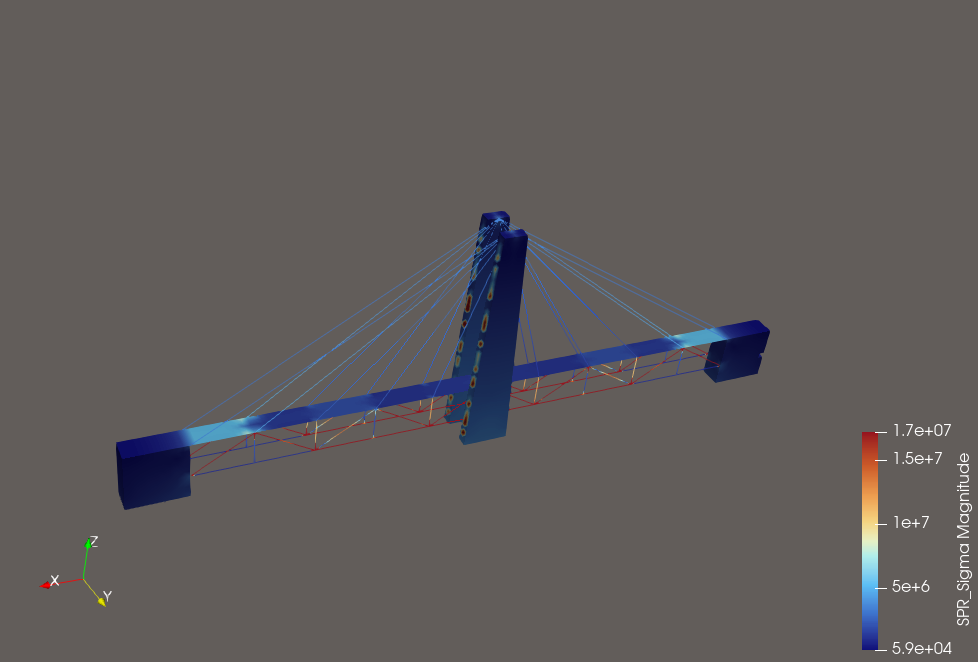
\includegraphics[width=0.92\textwidth]{应力云图.png}
    \caption{Bridge-1 应力云图}
    \label{fig:bridge1_stress_cloud}
\end{figure}

\begin{figure}[H]
    \centering
    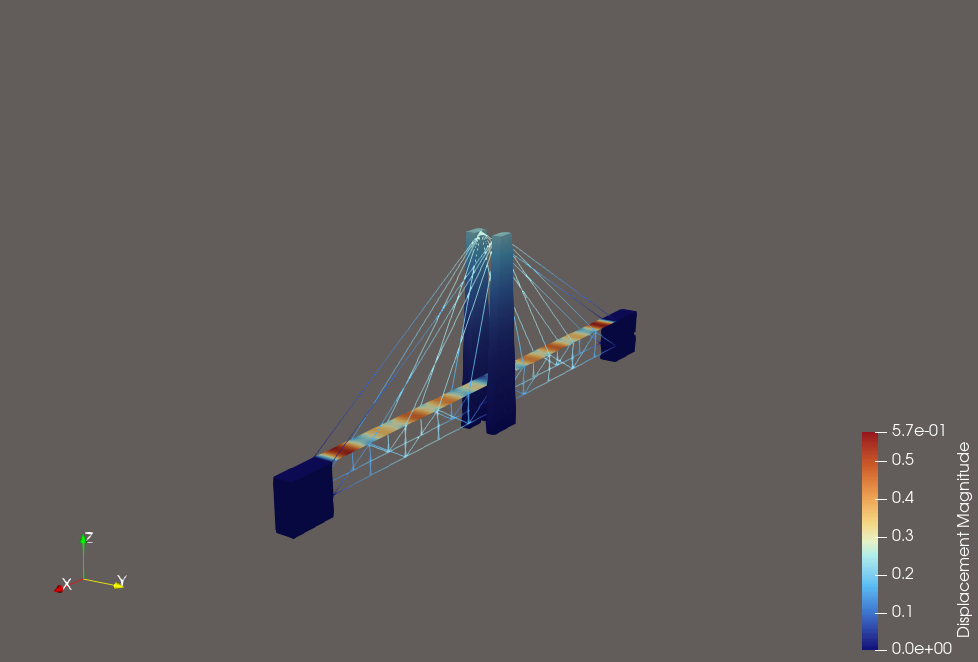
\includegraphics[width=0.92\textwidth]{位移云图.png}
    \caption{Bridge-1 位移云图}
    \label{fig:bridge1_displacement_cloud}
\end{figure}

\subsection{综合验证结论}

\begin{table}[H]
    \centering
    \caption{各单元验证结果汇总}
    \label{tab:verification_summary}
    \begin{tabular}{p{0.15\textwidth}p{0.20\textwidth}p{0.20\textwidth}p{0.30\textwidth}}
        \toprule
        单元 & 片单元检验 & 分片检验 & 收敛性表现\\
        \midrule
        Q4 & $\sigma_x$ 正确，单粗单元有寄生剪切 & 通过 & 粗网格剪切锁定，细网格恢复较好收敛\\
        Q4R & 中心应力正确，位移偏软 & 通过 & 显著减轻剪切锁定，粗网格精度高\\
        T3 & 精确表达常应力 & 通过 & 弯曲问题偏刚，收敛慢于 Q4\\
        Beam & 轴向/弯曲精确 & 精确 & 集中载荷下与网格无关的精确解\\
        H8 & $\sigma_x$ 正确 & 通过 & 粗网格剪切锁定，细网格收敛\\
        Plate & 弯矩/剪力精确 & 通过 & 选择性缩减积分避免剪切锁定，收敛良好\\
        \bottomrule
    \end{tabular}
\end{table}

% ============================================================
\section{任务分工与合作情况}

\begin{table}[H]
    \centering
    \caption{任务分工表}
    \label{tab:division}
    \begin{tabular}{p{0.20\textwidth}p{0.55\textwidth}p{0.15\textwidth}}
        \toprule
        成员 & 主要任务 & 完成情况\\
        \midrule
        王博淳 & 组长；实现 T3 常应变三角形单元，生成 T3 收敛性测试网格； MKL/PARDISO 求解模块配置与大规模算例加速 & 已完成\\
        聂锦浩 & 实现 Q4 全积分平面应力单元与 Q4R 缩减积分稳定化单元，完成片单元与分片检验；完成 Bridge-1 算例构建、验证、前后处理；报告修改 & 已完成\\
        袁彧诚 & 实现 Plate 四节点板弯曲单元，完成选择性缩减积分与板弯曲验证； MKL/PARDISO 求解模块配置与大规模算例加速 & 已完成\\
        陈 煜 & 实现 Beam 二维欧拉--伯努利框架单元，完成轴向拉伸与悬臂梁验证；撰写报告 & 已完成\\
        范滨珲 & 实现 H8 八节点六面体三维实体单元，完成分片检验与三维收敛分析；撰写报告 & 已完成\\
        \bottomrule
    \end{tabular}
\end{table}

团队合作过程中，首先统一输入数据格式和单元编号规范，然后分别实现各单元并进行独立调试；在单元片检验通过后，再统一进行分片检验和悬臂梁（板）收敛分析。最后对 Q4、Q4R、T3、Beam、H8 和 Plate 的数值结果进行横向比较，形成对各类单元性能的整体认识。

% ============================================================
\section{结论}

本文基于 STAP++ 程序完成了多种有限元单元的研发、验证和收敛性分析。主要结论如下：

\begin{enumerate}
    \item \textbf{程序框架清晰，适合单元扩展。}
    STAP++ 采用节点、材料、单元组、计算域、skyline 矩阵和求解器等模块化结构，单元扩展时只需实现统一接口并在单元工厂逻辑中注册即可。除原有 Bar 单元外，本文新增了 Q4/Q4R 平面四边形单元、T3 三角形单元、Beam 梁单元、H8 实体单元和 Plate 板单元五类单元功能，验证了框架的良好可扩展性。

    \item \textbf{Q4 全积分单元可以正确表达常应力状态。}
    Q4 单元在 $2\times2$ 分片检验中能够精确得到均匀拉伸理论应力，说明单元刚度矩阵和应力恢复实现正确。

    \item \textbf{Q4 单元在弯曲粗网格中存在剪切锁定。}
    悬臂梁算例中，$2\times1$ 网格的自由端挠度仅为解析解的 9.4\%，表明全积分双线性四边形单元在弯曲问题中会引入过大的寄生剪切刚度。随着网格加密，Q4 位移收敛率逐渐恢复，细网格阶段达到接近 $O(h^2)$ 的收敛阶。

    \item \textbf{Q4R 缩减积分稳定化单元显著改善弯曲性能。}
    Q4R 采用
    \[
        \Kmat=\Kmat_1+0.05(\Kmat_{\mathrm{full}}-\Kmat_1)
    \]
    的物理稳定化策略，既减轻剪切锁定，又避免纯缩减积分带来的奇异沙漏模式。在 $4\times2$ 网格下，Q4R 挠度误差仅为 11.6\%，明显优于 Q4 的 70.8\%。

    \item \textbf{T3 单元通过常应力检验，但弯曲问题中偏刚。}
    T3 常应变三角形单元可精确表达常应力场，因此片单元和分片检验均通过；但由于单元内部应变恒定，对弯曲应变场表达能力有限，在悬臂梁问题中收敛慢于 Q4。

    \item \textbf{Beam 单元在 Euler--Bernoulli 条件下给出精确解。}
    由于三次 Hermite 形函数恰好可以精确插值集中载荷下的梁挠度曲线，且刚度矩阵为解析精确矩阵，Beam 单元在所有测试网格下均给出与理论值误差小于 $0.01\%$ 的结果。

    \item \textbf{H8 三维单元存在剪切锁定，但随网格加密收敛。}
    H8 八节点六面体单元在粗网格弯曲问题中表现出与 Q4 类似的剪切锁定现象，$4\times2\times1$ 网格挠度仅为解析解的 28.8\%；随着网格加密逐步收敛，$32\times16\times1$ 网格达到 96.2\%。

    \item \textbf{Plate 单元通过选择性缩减积分有效避免剪切锁定。}
    Plate 四节点板单元将弯曲刚度与剪切刚度分离，弯曲部分采用 $2\times2$ 积分，剪切部分采用单点缩减积分。悬臂板算例表明，$4\times1$ 网格挠度即达到梁理论参考值的 96.5\%，收敛性能良好。

    \item \textbf{Bridge-1 工程算例验证了混合单元和大规模求解流程。}
    Bridge-1 默认输入为包含 4107 个节点、2884 个单元和 66 条可化简 MPC 方程的稳定版本；CMake 编译后的程序可通过 PARDISO 稀疏直接路径稳定求解，也可在完整输出需求下使用 skyline 直接法生成包含位移和应力表的 \texttt{Bridge-1.out}。最终桥面板位移向量中位误差为 $4.01\%$，满足 $5\%$ 优化目标；支撑梁误差接近目标，剩余差异主要集中在桥塔连接带。

    \item \textbf{工程应用建议。}
    对拉伸、压缩等常应力或近似常应力问题，Q4、T3 和 H8 均可使用；对以弯曲为主的平面问题，优先使用 Q4R 或足够细密的 Q4 网格；对框架结构，Beam 单元可在粗网格下获得精确结果；对板弯曲问题，Plate 单元配合选择性缩减积分是经济高效的选择；对三维实体弯曲问题，H8 需要较细密的网格才能克服剪切锁定，可考虑使用缩减积分或高阶单元。
\end{enumerate}

综上，本次课程设计完成了从有限元单元公式推导、程序实现、输入数据构造到数值验证和收敛性分析的完整流程，加深了对有限元程序内部实现机制、不同维度单元数值特性以及分片检验意义的理解。

本次课程设计的代码实现、测试数据和报告文档均已上传至 GitHub 仓库 \url{https://github.com/wangbc1124/STAPpp}
% ============================================================
\begin{thebibliography}{99}

\bibitem{zhang2007}
张雄，王天舒.
\newblock 计算动力学.
\newblock 北京：清华大学出版社，2007.

\bibitem{zhang2015}
张雄，王天舒，刘岩.
\newblock 计算动力学：第2版.
\newblock 北京：清华大学出版社，2015.

\bibitem{zienkiewicz}
Zienkiewicz O. C., Taylor R. L., Zhu J. Z.
\newblock The Finite Element Method: Its Basis and Fundamentals.
\newblock 7th ed. Oxford: Butterworth-Heinemann, 2013.

\bibitem{hughes}
Hughes T. J. R.
\newblock The Finite Element Method: Linear Static and Dynamic Finite Element Analysis.
\newblock Mineola: Dover Publications, 2000.

\bibitem{bathe}
Bathe K. J.
\newblock Finite Element Procedures.
\newblock Englewood Cliffs: Prentice Hall, 1996.

\bibitem{gb3102}
国家技术监督局.
\newblock GB 3102.11--1993 物理科学和技术中使用的数学符号.
\newblock 北京：中国标准出版社，1993.

\bibitem{stappp}
Computational Dynamics Laboratory, Tsinghua University.
\newblock STAP++ finite element code and documentation.
\newblock \url{https://xzhang66.github.io/stappp/index.html}.

\bibitem{abaqus}
Dassault Systèmes.
\newblock Abaqus Analysis User's Guide.
\newblock Providence, RI: Dassault Systèmes Simulia Corp.

\end{thebibliography}

\end{document}
